\documentclass[10pt,a4paper, margin=1in]{article}
\usepackage{fullpage}
\usepackage{amsfonts, amsmath, pifont}
\usepackage{amsthm}
\usepackage{graphicx}
\usepackage{float}
\usepackage{listings}
\usepackage{color}
\usepackage{steinmetz}

\lstset{frame=tb,
  language=Python,
  aboveskip=3mm,
  belowskip=3mm,
  showstringspaces=false,
  columns=flexible,
  basicstyle={\small\ttfamily},
  numbers=none,
  numberstyle=\tiny\color{gray},
  keywordstyle=\color{blue},
  commentstyle=\color{green},
  stringstyle=\color{red},
  breaklines=true,
  breakatwhitespace=true,
  tabsize=3
}

\usepackage{tkz-euclide}
\usepackage{tikz}
\usepackage{pgfplots}
\pgfplotsset{compat=1.13}

\usepackage{geometry}
 \geometry{
 a4paper,
 total={210mm,297mm},
 left=10mm,
 right=10mm,
 top=10mm,
 bottom=16mm,
 }
 % Write both of your names here. Fill exxxxxxx with your ceng mail address.
 \author{
  Akçan, Batuhan\\
  \texttt{e2580181@ceng.metu.edu.tr}
  \and
  Sönmezer, Mert\\
  \texttt{e2516920@ceng.metu.edu.tr}
}

\title{CENG 384 - Signals and Systems for Computer Engineers \\
Spring 2024 \\
Homework 3}
\begin{document}
\maketitle



\noindent\rule{19cm}{1.2pt}

\begin{enumerate}

\item %write the solution of q1
We know the formula
$$x(t) = \sum_{k=-\infty}^{\infty} a_k e^{jkw_0t}.$$
And, we know that
$$T=4 \; \rightarrow w_0 = \frac{2\pi}{4} = \frac{\pi}{2}.$$
Thus, $\; x(t) \;$ becomes
$$x(t) = \sum_{k=-\infty}^{\infty} a_k e^{jk\frac{\pi}{2}t}$$
$$=
\begin{cases}
    \sum_{k=-\infty}^{\infty}-e^{jk\frac{\pi}{2}t} & \text{k is even}\\
    \sum_{k=-\infty}^{\infty}e^{jk\frac{\pi}{2}t} & \text{k is odd}
\end{cases}
$$
$$=\sum_{k=-\infty}^{\infty}a_{2k}e^{jk\pi t}+\sum_{k=-\infty}^{\infty}a_{2k+1}e^{j(2k+1)\pi t}$$
$$=-\sum_{k=-\infty}^{\infty}e^{jk\pi t}+e^{j\frac{\pi}{2} t}\sum_{k=-\infty}^{\infty}e^{jk\pi t}$$
$$=(e^{j\frac{\pi}{2}t} - 1)\sum_{k=-\infty}^{\infty}e^{jk\pi t}$$
$$= ... \; e^{-j3\frac{\pi}{2} t} - e^{-j\pi t}+e^{-j\frac{\pi}{2}t}-1+e^{j\frac{\pi}{2}t}-e^{j\pi t} + e^{j3\frac{\pi}{2}t} - \; ...$$

\item %write the solution of q2  
    \begin{enumerate}
    % Write your solutions in the following items.
    \item %write the solution of q2a
    We know the formula
    $$a_k = \frac{1}{T}\int_{T} x(t)e^{-jkw_0t}dt.$$
    And, we know that
    $$T=4 \; \rightarrow \; w_0 = \frac{2\pi}{4} = \frac{\pi}{2}.$$
    Hence, we have
    $$a_k = \frac{1}{4}\int_{0}^{2} 2te^{-jk\frac{\pi}{2}t}dt + \frac{1}{4}\int_{2}^{4}(4-t)e^{-jk\frac{\pi}{2}t}dt$$
    $$= \frac{1}{2}\int_{0}^{2}te^{-jk\frac{\pi}{2}t}dt + \int_{2}^{4}e^{-jk\frac{\pi}{2}t}dt - \frac{1}{4}\int_{2}^{4}te^{-jk\frac{\pi}{2}t}dt$$
    $$= \frac{1}{2}I_1 + I_2 - \frac{1}{4}I_3.$$
    For $\; I_1, \;$ let $\; u=t, \; dv=e^{-jk\frac{\pi}{2}t}dt. \;$ Then, $\; du=dt, \; v=\frac{-2}{jk\pi}e^{-jk\frac{\pi}{2}t}. \;$
    By Integration By Parts, we have
    $$I_1 = uv - \int_{0}^{2}vdu = \frac{-2t}{jk\pi} - \int_{0}^{2}\frac{-2}{jk\pi}e^{-jk\frac{\pi}{2}t}dt$$
    $$= \frac{-2t}{jk\pi} + \frac{-4}{j^2k^2\pi^2}e^{-jk\frac{\pi}{2}t} \Bigm|_{0}^{2} = \frac{-2t}{jk\pi}+\frac{4}{k^2\pi^2}(e^{-jk\pi}-1).$$
    Calculating $\; I_2, \;$
    $$I_2 = \int_{2}^{4}e^{-jk\frac{\pi}{2}t}dt = \frac{-2}{jk\pi}e^{-jk\frac{\pi}{2}t} \Bigm|_{2}^{4} = \frac{-2}{jk\pi}(e^{-jk2\pi}-e^{-jk\pi}).$$
    Since $\; I_3 \;$ is similar to $\; I_1, \;$ we can directly write
    $$I_3 = \frac{-2t}{jk\pi} + \frac{4}{k^2\pi^2}(e^{-jk2\pi} - e^{-jk\pi}).$$
    Thus,
    $$a_k = \frac{1}{2}I_1 + I_2 - \frac{1}{4}I_3$$
    $$= \frac{-t}{jk\pi} + \frac{2}{k^2\pi^2}e^{-jk\pi} - \frac{2}{k^2\pi^2} - \frac{2}{jk\pi}e^{-jk2\pi} + \frac{2}{jk\pi}e^{-jk\pi} + \frac{t}{2jk\pi} - \frac{1}{k^2\pi^2}e^{-jk2\pi} + \frac{1}{k^2\pi^2}e^{-jk\pi}$$
    $$= \frac{-t}{2jk\pi} - \frac{2}{k^2\pi^2} + \frac{2}{jk\pi}(e^{-jk\pi} - e^{-jk2\pi}) + \frac{1}{k^2\pi^2}(3e^{-jk\pi} - e^{-jk2\pi})$$
    $$= \frac{2}{jk\pi}(e^{-jk\pi} - e^{-jk2\pi} - \frac{t}{4}) + \frac{1}{k^2\pi^2}(3e^{-jk\pi} - e^{-jk2\pi} - 2).$$\vspace{0.3cm}\\
    
    \item %write the solution of q2b
    The Differentiation Property states that, if
    $$x(t) \leftrightarrow a_k$$
    then,
    $$\frac{dx(t)}{dt} \leftrightarrow jkw_0a_k.$$
    Applying this property, we get
    $$a_k = \frac{jk\pi}{2}\frac{2}{jk\pi}(e^{-jk\pi}-e^{-jk2\pi}-\frac{t}{4}) + \frac{jk\pi}{2}\frac{1}{k^2\pi^2}(3e^{-jk\pi}-e^{-jk2\pi}-2)$$
    $$= e^{-jk\pi}-e^{-jk2\pi}-\frac{t}{4}+\frac{j}{2k\pi}(3e^{-jk\pi}-e^{-jk2\pi}-2).$$\vspace{0.3cm}\\
    \end{enumerate}

\item %write the solution of q3
    \begin{enumerate}
    % Write your solutions in the following items.
    \item %write the solution of q3a
    Let's start with the first DT signal $\; x_1[n]. \;$ Its period can be found as follows:
        \begin{align*}
            cos(\frac{\pi}{2}n) &= cos(\frac{\pi}{2}n+\frac{\pi}{2}N) \\ 
            \frac{\pi}{2}n+2\pi m &= \frac{\pi}{2}n+\frac{\pi}{2}N
        \end{align*}
    Then, the equations above drives us to find $m=1$ and $N=4$. According to Table 7.2 in the book, the spectral coefficients of $\; x_1[n], \;$ which we define as $\; a_k \;$ will be as follows:
    $$a_k = 
        \begin{cases}
            \frac{1}{2} & k=\pm 1, \pm 1 \pm 4, \pm 1 \pm 8\\
            0 & \text{otherwise}
        \end{cases}
    $$
    When applying the same process for $\; x_2[n] \;$, the following is obtained:
        \begin{align*}
            sin(\frac{\pi}{2}n) &= sin(\frac{\pi}{2}n+\frac{\pi}{2}N) \\ 
            \frac{\pi}{2}n+2\pi m &= \frac{\pi}{2}n+\frac{\pi}{2}N
        \end{align*}
    Then, $m$ and $N$ values are 1 and 4 respectively. According to Table 7.2 in the book, the spectral coefficients of $\; x_2[n], \;$ which we define as $\; b_k \;$ will be as follows:
    $$b_k = 
        \begin{cases}
             \frac{1}{2j} & k=\pm 1, \pm 1 \pm 4, \pm 1 \pm 8, ...\\
            -\frac{1}{2j} & k=-1, -1 \pm 4, -1 \pm 8, ...
        \end{cases}
    $$
    As in the question, $\; x_3[n] \;$ is the product of the first two signals. After the following algebraic manipulation, we get a sine-based signal.
    $$cos(\frac{\pi}{2}n)sin(\frac{\pi}{2}n) = \frac{1}{2}sin(\pi n)$$
    Utilizing the method of linearity and Table 7.2 in the book, $\; c_k \;$ is found below.
    $$c_k = 
        \begin{cases}
            \frac{1}{4j} & k=\pm 1, \pm 1 \pm 2, \pm 1 \pm 4, ...\\
            -\frac{1}{4j} & k=-1, -1 \pm 2, -1 \pm 4, ...
        \end{cases}
    $$\vspace{0.3cm}\\
    
    \item %write the solution of q3b
    The multiplication property states that, multiplication operation in time domain corresponds to convolution operation in frequency domain. Using this fact, we can define $\; c_k \;$ as follows:
        \begin{align*}
            x_3[n] &\leftrightarrow c_k \\
            x_1[n]x_2[n] &\leftrightarrow a_k * b_k
        \end{align*}
    So, we have
    $$c_k = \sum_{l=-\infty}^{\infty}a_lb_{k-l}.$$
    Using the spectral coefficients we found in previous part, this sum is equal to
    $$c_k=\frac{1}{2}b_{k-1}+\frac{1}{2}b_{k-3}$$
     Notice that the magnitude of $c_k$ is half compared to $b_k$, and its frequency is twice $b_k$'s since the two terms in the expression. Then, $c_k$ is below.
    $$c_k = 
        \begin{cases}
            \frac{1}{4j} & k=\pm 1, \pm 1 \pm 2, \pm 1 \pm 4, ...\\
            -\frac{1}{4j} & k=-1, -1 \pm 2, -1 \pm 4, ...
        \end{cases}
    $$
    To wrap up, when comparing the $c_k$ signals found in this part and the previous part, they are identical.
    \end{enumerate}\vspace{0.3cm}

\item %write the solution of q4
Using the linearity property, we can split $a_k$ into two terms, as
$\; a_k = a_k^{(1)}+a_k^{(2)}$
where $\; a_k^{(1)} = cos(k\frac{\pi}{3}) \;$ and $\; a_k^{(2)} = cos(k\frac{\pi}{4}). \;$ Each of them corresponds a signal in time domain. Those are defined below.
    \begin{align*}
        x_1[n] \leftrightarrow a_k^{(1)} \\
        x_2[n] \leftrightarrow a_k^{(2)}
    \end{align*}
The linearity property implies that,
$$x[n] = x_1[n]+x_2[n] \leftrightarrow a_k = a_k^{(1)}+a_k^{(2)}$$
The spectral coefficients $a_k^{(1)}$ and $a_k^{(2)}$ can be written in terms of complex exponential functions.
    \begin{align*}
        a_k^{(1)} = cos(k\frac{\pi}{3}) = \frac{e^{jk\frac{\pi}{3}}+e^{-jk\frac{\pi}{3}}}{2} \\
        a_k^{(2)} = cos(k\frac{\pi}{4}) = \frac{e^{jk\frac{\pi}{4}}+e^{-jk\frac{\pi}{4}}}{2}
    \end{align*}
The angular frequency of $\; a_k^{(1)} \;$ and $\; a_k^{(2)} \;$ are $\; \frac{\pi}{3} \;$ and $\; \frac{\pi}{4} \;$ respectively. The analysis equations for both can be written as follows:
    \begin{align*}
        a_k^{(1)} = \frac{1}{6}\sum_{n=-2}^{3}x_1[n]e^{-jk\frac{\pi}{3}n} = \frac{1}{2}e^{jk\frac{\pi}{3}} + \frac{1}{2}e^{-jk\frac{\pi}{3}} \\
        a_k^{(2)} = \frac{1}{8}\sum_{n=-3}^{4}x_2[n]e^{-jk\frac{\pi}{4}n} = \frac{1}{2}e^{jk\frac{\pi}{4}} + \frac{1}{2}e^{-jk\frac{\pi}{4}} \\
    \end{align*}
Comparing the left hand side and the right hand side of the equations above,
\begin{align*}
    x_1[1] = x_1[-1] = 3 \rightarrow N=6 \\
    x_1[1] = x_1[-1] = 4 \rightarrow N=8 
\end{align*}
Note that $x[n]$ is periodic, and its period is the LCM of $x_1[n]$'s and $x_2[n]$'s, which is 24. In the interval $-1\leq n\leq 23$, $x_1[n]$ and $x_2[n]$ are written as,
    \begin{align*}
        x_1[-1] = x_1[1] = x_1[5] = x_1[7] = x_1[11] = x_1[13] = x_1[17] = x_1[19] = x_1[23] = 3\\
        x_2[-1] = x_2[1] = x_2[7] = x_2[9] = x_2[15] = x_2[17] = x_2[23] = 4
    \end{align*}
Hence, $x[n]$ can be written as follows:
    \begin{align*}
        x[n] &= x_1[n] + x_2[n] \\
        x[n] &= 7\delta[n+1]+7\delta[n-1]+3\delta[n-5]+7\delta[n-7]+4\delta[n-9]+3\delta[n-11]+\\
        &3\delta[n-13]+4\delta[n-15]+7\delta[n-17]+3\delta[n-19]+7\delta[n-23]
    \end{align*}
Notice that $\; x[n] \;$ is a periodic function, where $\; x[n]=x[n\pm 24] \;$ for all $\; n \in \mathbb{Z}.$\vspace{0.3cm}\\

\item %write the solution of q5  
    \begin{enumerate}   
    % Write your solutions in the following items.
    \item %write the solution of q5a
    Notice that the signal is a discrete time signal. Let's apply the steps to find its period.
    \begin{align*}
        &x[n]=sin(\frac{6\pi}{13}n+\frac{\pi}{2})\\
        &sin(\frac{6\pi}{13}n+\frac{\pi}{2}) = sin(\frac{6\pi}{13}n+\frac{6\pi}{13}N+\frac{\pi}{2}) \\
        &\frac{6\pi}{13}n+\frac{\pi}{2}+2\pi m =\frac{6\pi}{13}n+\frac{6\pi}{13}N+\frac{\pi}{2}
    \end{align*}
    Then, we found that $N=13$ for $m=3$. That drives us $\omega_0=\frac{2\pi}{N}m=\frac{6\pi}{13}.$\vspace{0.3cm}\\
    
    \item %write the solution of q5b
    From Table 7.2, we see that spectral coefficients of $x'[n]=sin(\omega_0n)$ for $\omega_0=\frac{6\pi}{13}$ is,
    $$a'_k = 
        \begin{cases}
             \frac{1}{2j} & k=\pm 3, \pm 3 \pm 13, \pm 3 \pm 26, ...\\
            -\frac{1}{2j} & k=-3, -3 \pm 13, -3 \pm 26, ...
        \end{cases}
    $$
    Time-shifting property of DT Fourier Series states that, the time shift operation comes along with a multiplicative exponential factor in the frequency domain.
    \begin{align*}
        x[n]&=x'[n-n_0] \leftrightarrow a'_ke^{-jk\omega_0n_0} \\
        x[n]&=sin(\frac{6\pi}{13}n+\frac{\pi}{2})=sin(\frac{6\pi}{13}(n+\frac{13}{12}))
    \end{align*}
    Hence, $n_0=-\frac{13}{12}$. Replacing the values, we obtain
    $$a_k = 
        \begin{cases}
            \frac{1}{2j}e^{jk\frac{\pi}{2}} & k=\pm 3, \pm 3 \pm 13, \pm 3 \pm 26, ...\\
            -\frac{1}{2j}e^{jk\frac{\pi}{2}} & k=-3, -3 \pm 13, -3 \pm 26, ...
        \end{cases}
    $$
    Since $\; e^{\frac{j\pi}{2}}=j \;$ and $\; e^{\frac{-j\pi}{2}} = -j \;$, we can rewrite $\; a_k \;$ as
    $$a_k =
        \begin{cases}
            \frac{1}{2j}j^k & k=\pm 3, \pm 3 \pm 13, \pm 3 \pm 26, ...\\
            \frac{-1}{2j}(-j)^k & k=-3, -3 \pm 13, -3 \pm 26, ...
        \end{cases}
    $$
    As we can see, $\;a_k\;$ always takes the values $\; \pm\frac{1}{2j}\;$ and $\; \pm\frac{1}{2}, \;$ of which magnitude are $\; \frac{1}{2}. \;$ Hence, the magnitude spectrum is,
    $$|a_k| = \frac{1}{2} \hspace{0.2cm} \text{for} \hspace{0.2cm} k=\pm 3, \pm 3 \pm 13, \pm 3 \pm 26, ...$$
    and the phase spectrum is,
    $$\phase{a_k} =
        \begin{cases}
            (k-1)\frac{\pi}{2} \hspace{0.2cm} \text{for} \hspace{0.2cm} k=\pm 3, \pm 3 \pm 13, \pm 3 \pm 26, ...\\
            -(k-1)\frac{\pi}{2} \hspace{0.2cm} \text{for} \hspace{0.2cm} k=-3, -3 \pm 13, -3 \pm 26, ...
        \end{cases}
    $$
    Here are the plots:
    \begin{figure}[htbp]
        \centering
            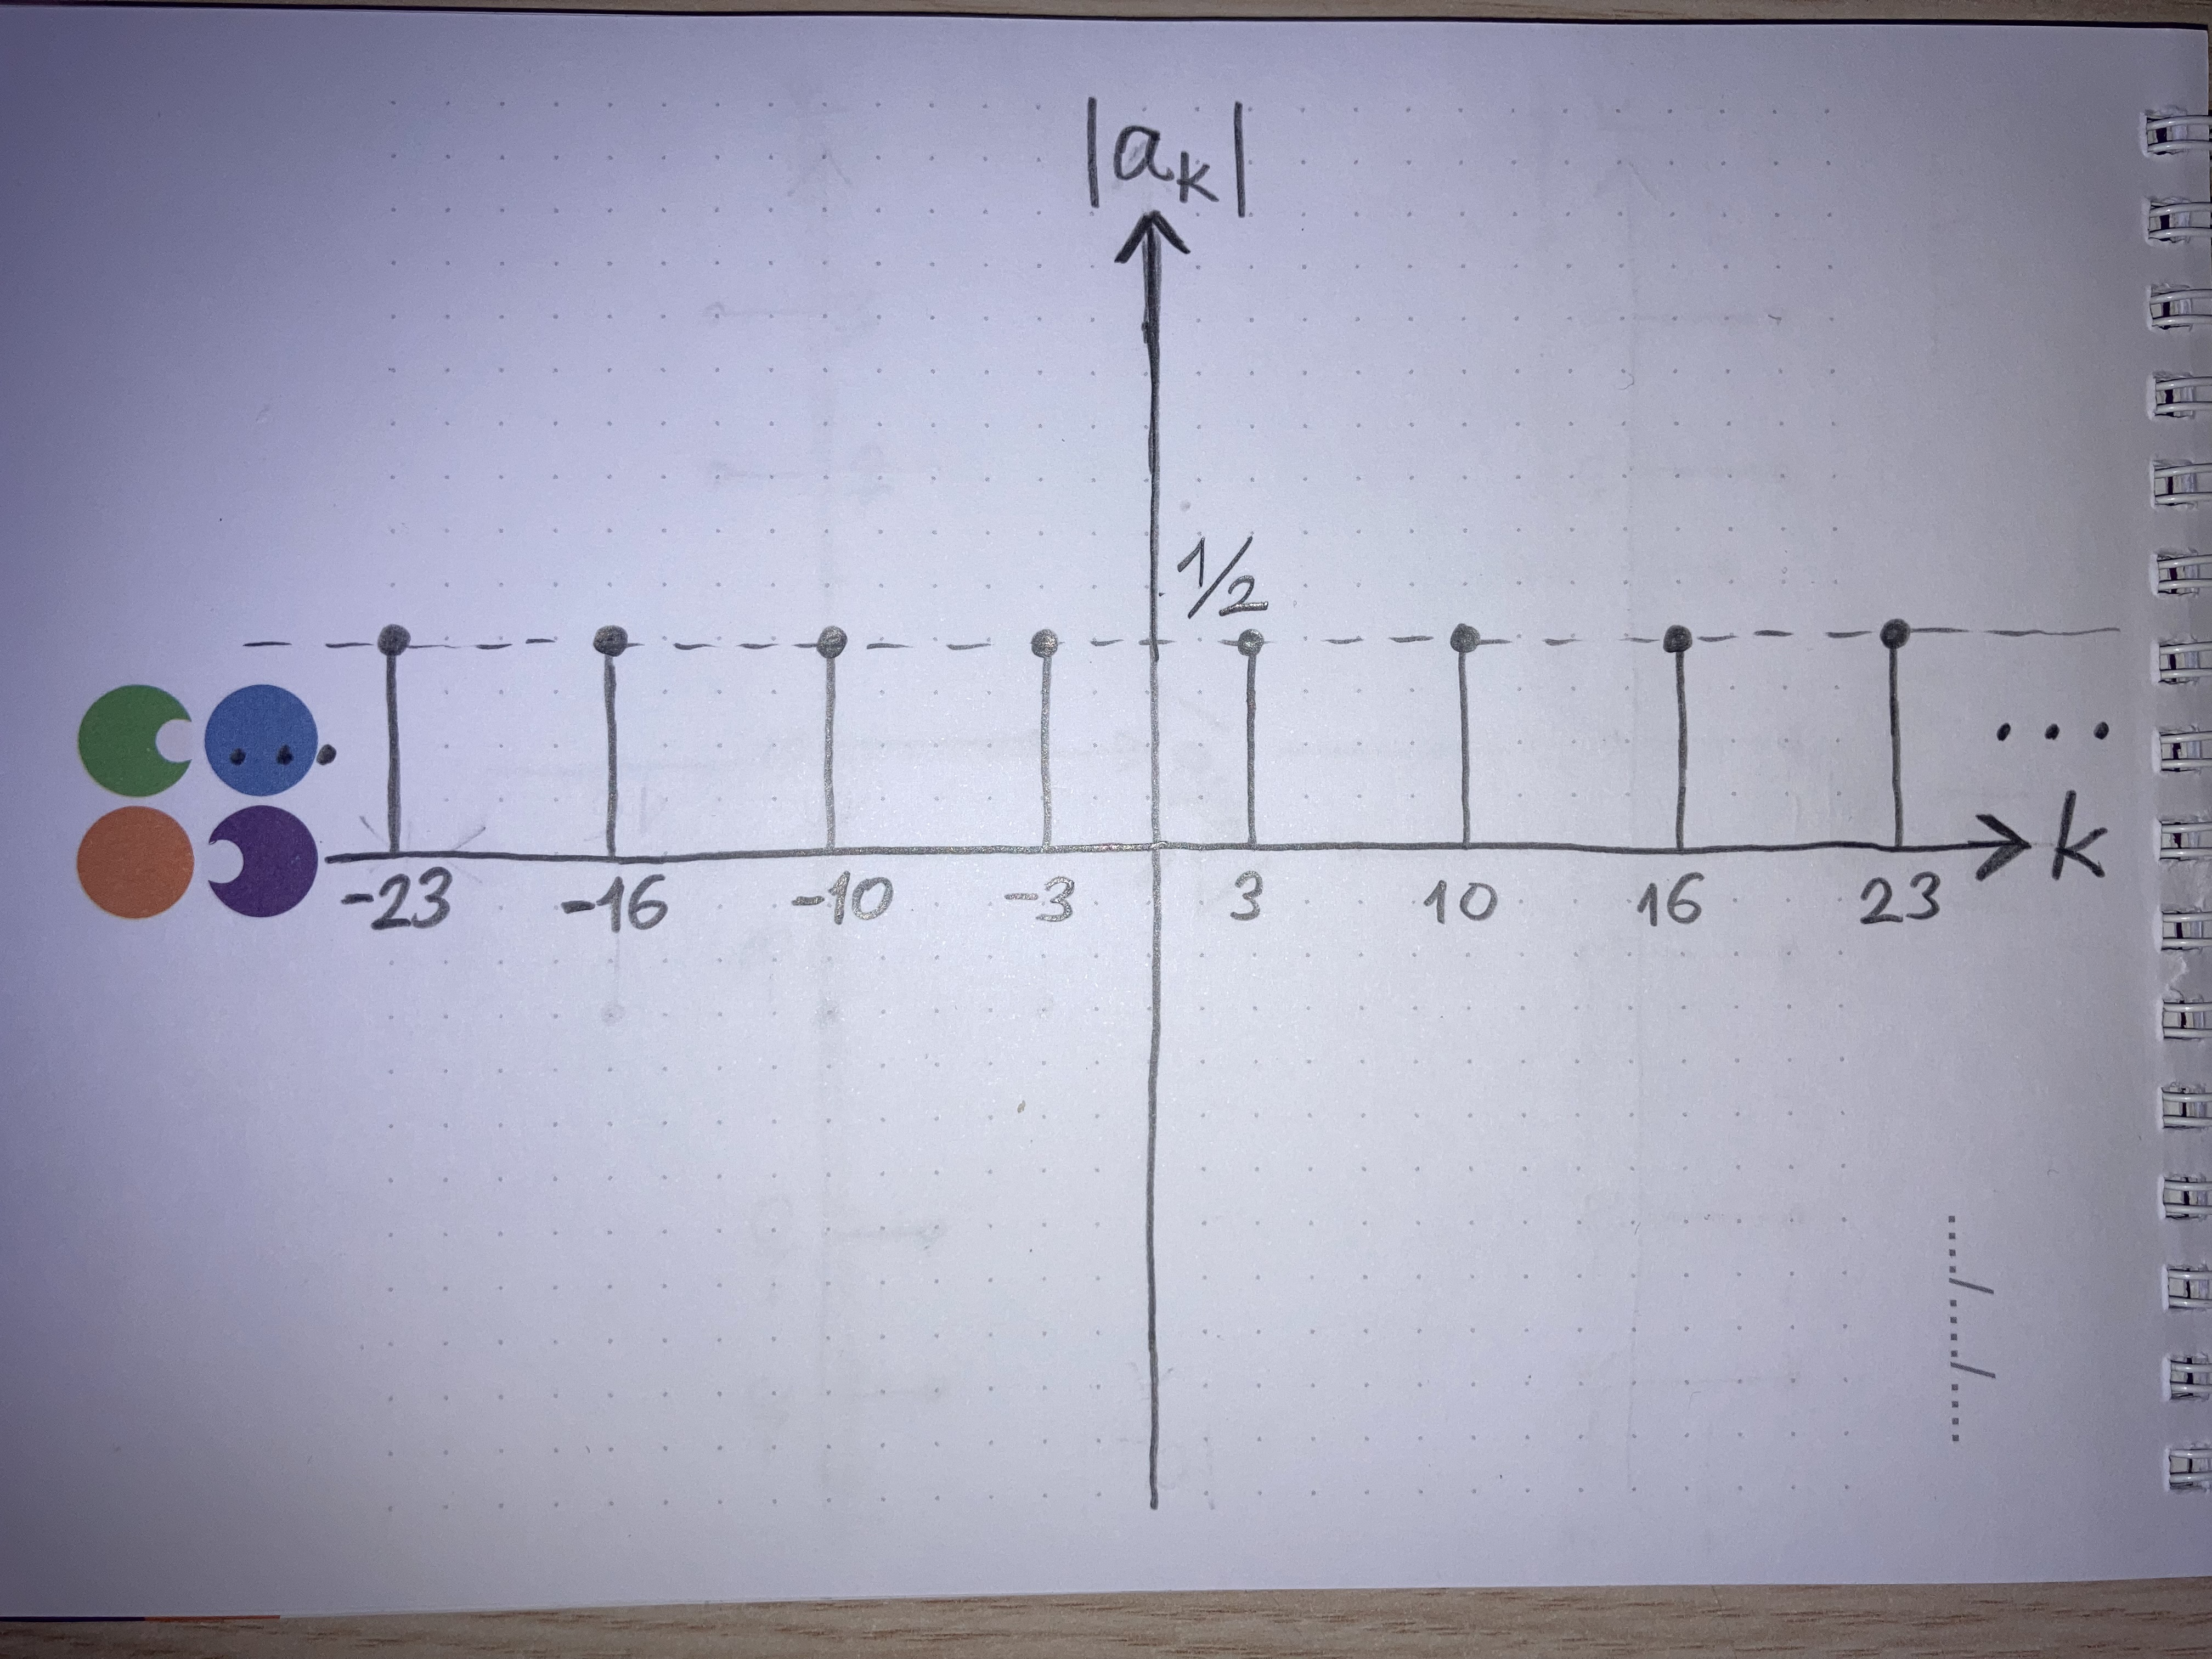
\includegraphics[width=1\textwidth]{q5b_magnitude.jpg}
            \caption{Magnitude plot}
            \label{fig:q5b_mag}
    \end{figure}

    \begin{figure}[htbp]
        \centering
            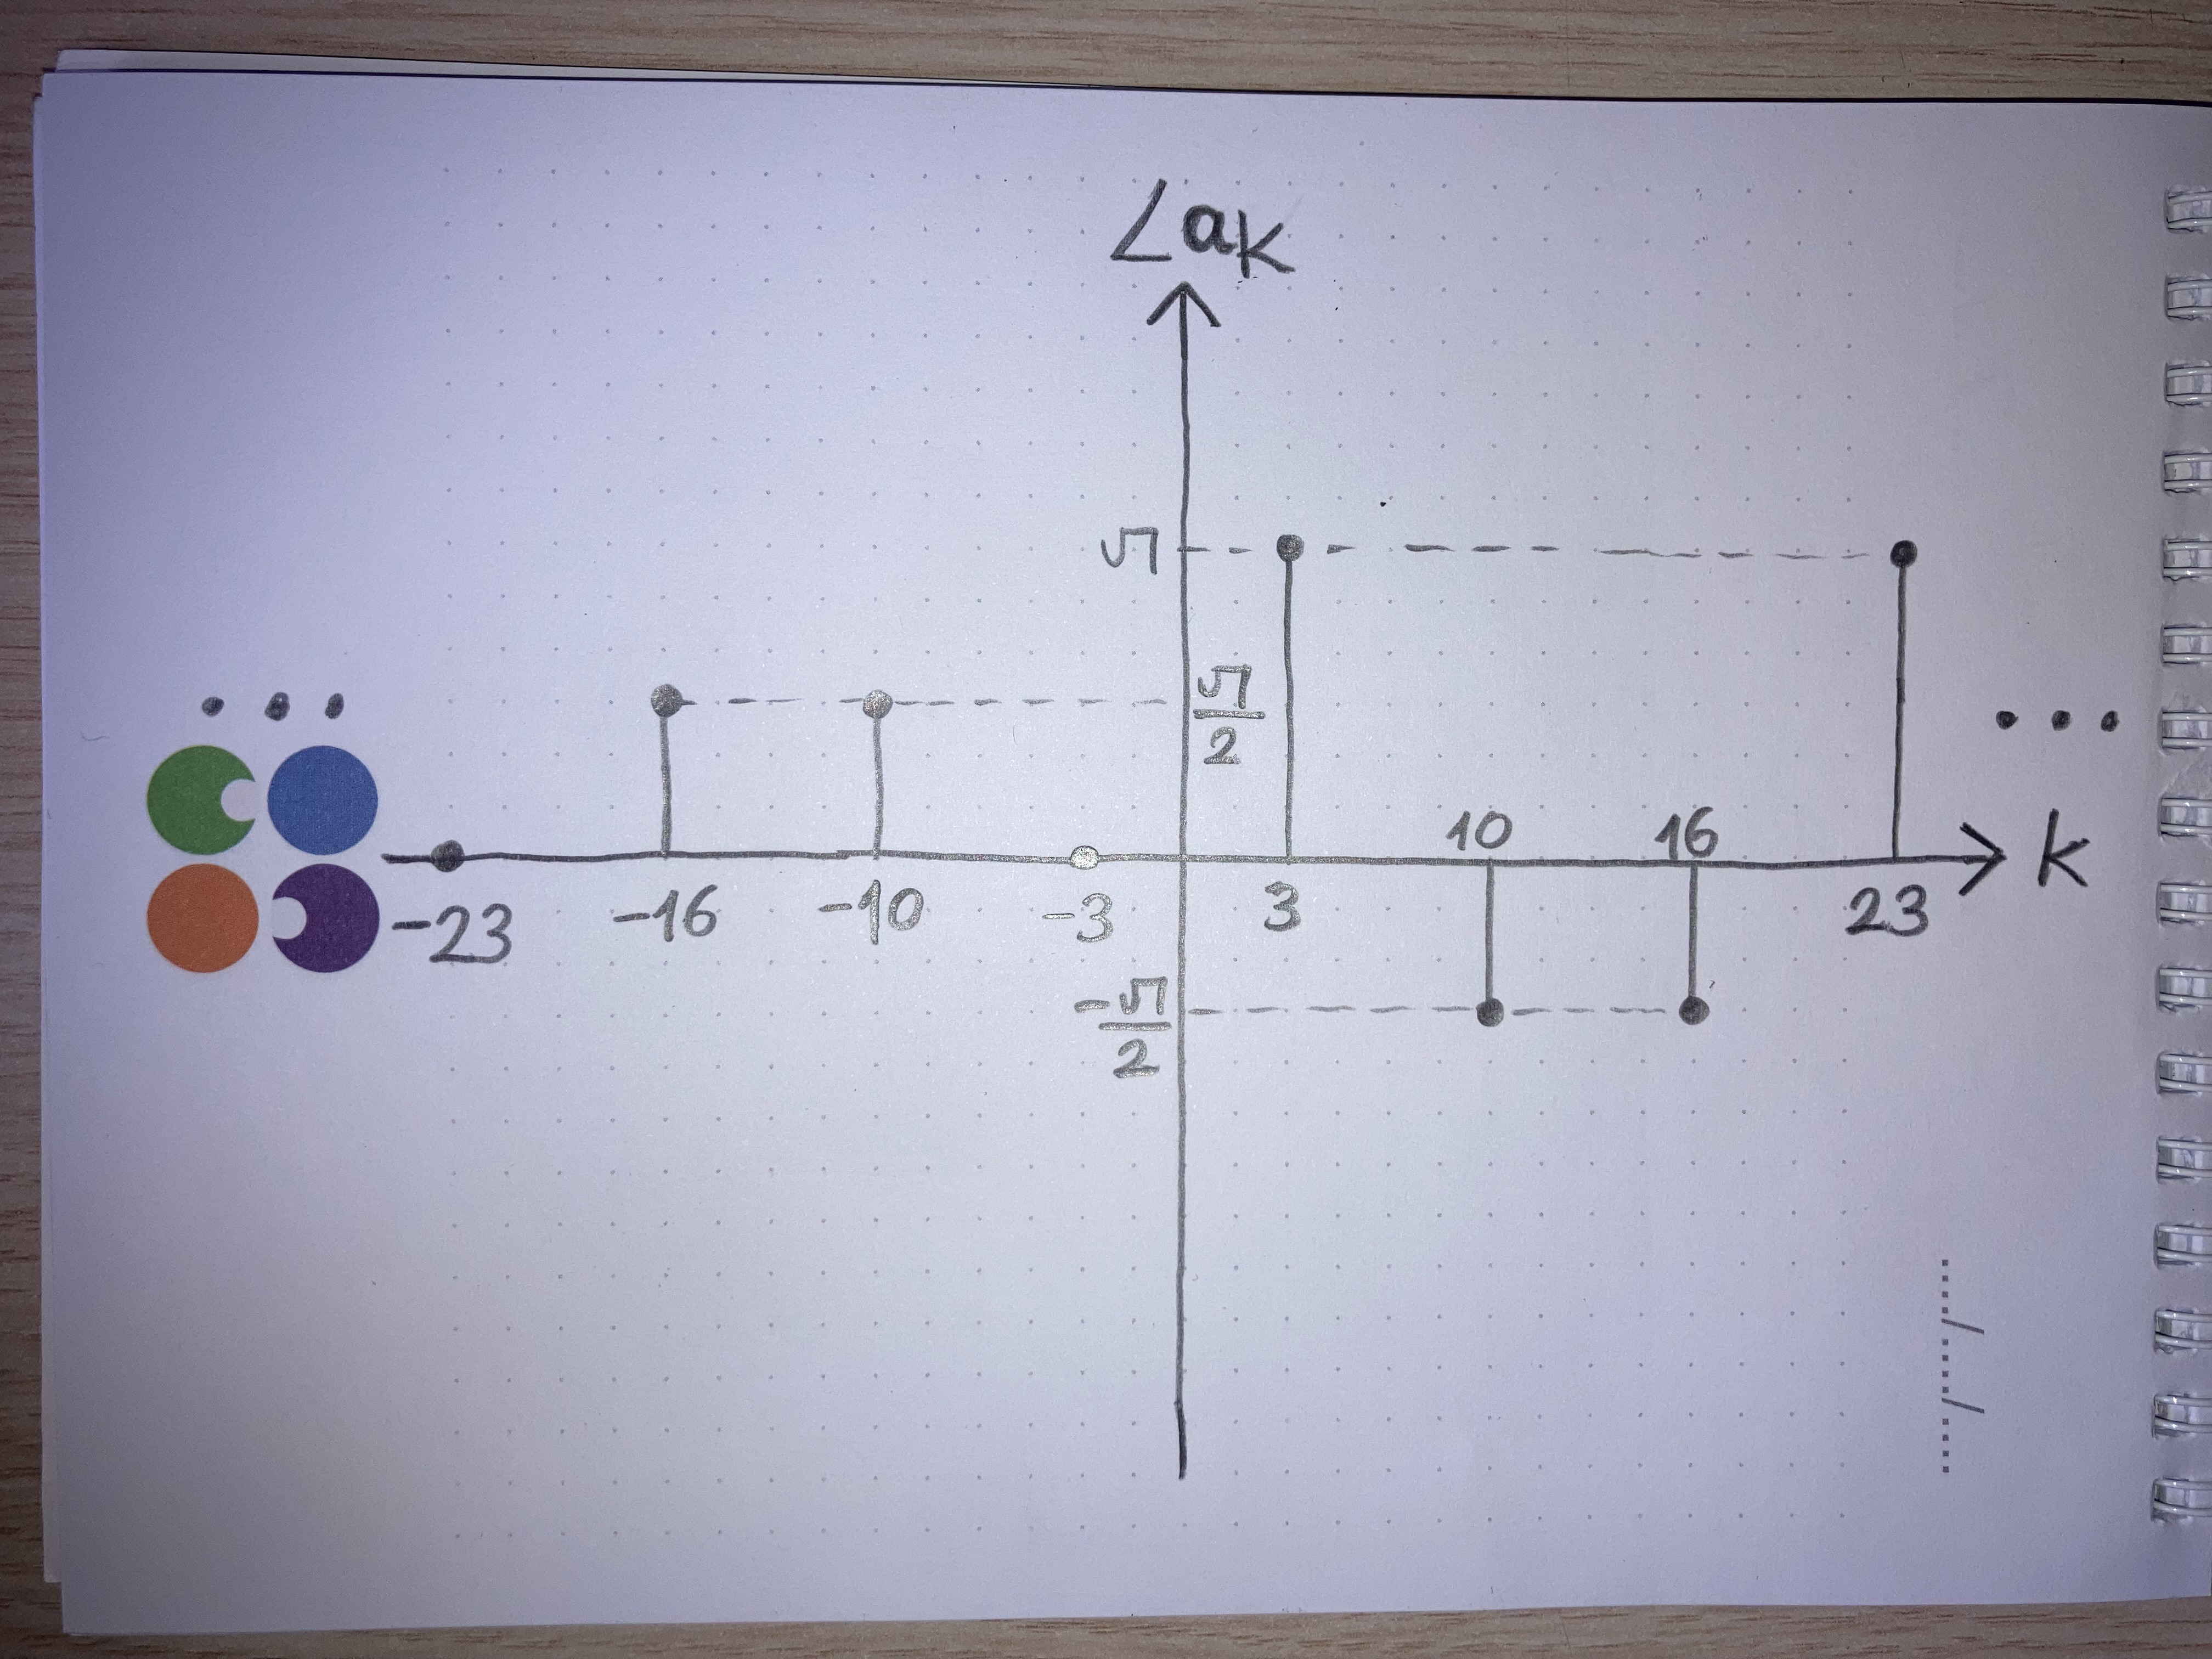
\includegraphics[width=1\textwidth]{q5b_phase.jpg}
            \caption{Phase plot}
            \label{fig:q5b_pha}
    \end{figure}
    \end{enumerate}

\newpage
    
\item %write the solution of q6
    \begin{enumerate}
    % Write your solutions in the following items.
    \item %write the solution of q6a
    We have
    $$H(jw) = \frac{1}{3+4jw} = \frac{1}{4}\frac{1}{\frac{3}{4}+jw}.$$
    We know that
    $$\frac{1}{a+jw} \leftrightarrow e^{-at}u(t).$$
    Therefore,
    $$\frac{1}{\frac{3}{4}+jw} \leftrightarrow e^{\frac{-3t}{4}}u(t).$$
    By Linearity Property of Fourier Transform, we get
    $$H(jw) = \frac{1}{4}\frac{1}{\frac{3}{4}+jw} \leftrightarrow \frac{1}{4}e^{\frac{-3t}{4}}u(t).$$\vspace{0.3cm}\\
    
    \item %write the solution of q6b
    By Convolution Property of Fourier Transform,
    $$y(t) = x(t) \ast h(t) \; \leftrightarrow \; Y(jw) = X(jw)H(jw).$$
    We know the following property:
    $$e^{-at}u(t) \; \leftrightarrow \; \frac{1}{a+jw}.$$
    Thus, we have
    $$Y(jw) = \frac{1}{5+jw}-\frac{1}{10+jw} = \frac{5}{(10+jw)(5+jw)} = X(jw)H(jw).$$
    Hence,
    $$X(jw) = \frac{Y(jw)}{H(jw)} = \frac{\frac{5}{(10+jw)(5+jw)}}{\frac{1}{3+4jw}} = \frac{15+20jw}{(10+jw)(5+jw)}.$$
    To find the $x(t)$, the partial fraction method can be applied.
    $$\frac{15+20jw}{(10+jw)(5+jw)}=\frac{A}{10+jw}+\frac{B}{5+jw}.$$
    After some algebraic operations, we obtain the following equations:
    \begin{align*}
        A+B&=20\\
        5A+10B&=15\\
        A=37 \hspace{0.2cm} \text{and} \hspace{0.2cm} B&=-17
    \end{align*}
    Then, the expression below is obtained,
    $$X(jw)=\frac{37}{10+jw}+\frac{-17}{5+jw}.$$
    Since we know the conversion formula, $x(t)$ will be as follows:
    $$X(jw)\leftrightarrow x(t)=(37e^{-10t}-17e^{-5t})u(t).$$
    \end{enumerate}
    
\item %write the solution of q7    
In order to find $\;T,$\vspace{0.3cm}\\
Fundamental period of $\; cos(\frac{\pi t}{3}) = \frac{2\pi}{\frac{\pi}{3}} = 6.$\vspace{0.3cm}\\
Fundamental period of $\; 2cos(\pi t + \frac{\pi}{2}) = \frac{2\pi}{\pi} = 2.$\vspace{0.3cm}\\
Since they are added, their LCM gives the fundamental period of $\; x(t), \;$ which is $\; T=6.$\vspace{0.3cm}\\
Therefore, $\; w_0 = \frac{2\pi}{T} = \frac{\pi}{3}.$\vspace{0.3cm}\\
Rewrite $\; x(t) \;$ by using Euler's Formula:
$$x(t) = \frac{1}{2}e^{\frac{j\pi t}{3}} + \frac{1}{2}e^{\frac{-j\pi t}{3}} + e^{j(\pi t + \frac{\pi}{2})} + e^{-j(\pi t + \frac{\pi}{2})}.$$\vspace{0.3cm}\\
Since $\; e^{\frac{j\pi}{2}} = cos(\frac{j\pi}{2}) + jsin(\frac{j\pi}{2}) = 0 + j = j \;$ and $\; e^{\frac{-j\pi}{2}} = cos(\frac{-j\pi}{2}) + jsin(\frac{-j\pi}{2}) = 0 - j = -j, \;$ we have
$$x(t) = \frac{1}{2}e^{\frac{j\pi t}{3}} + \frac{1}{2}e^{\frac{-j\pi t}{3}} + je^{j\pi t} - je^{-j\pi t}.$$\vspace{0.3cm}\\
We know the formula
$$x(t) = \sum_{k=-\infty}^{\infty} a_k e^{-jkw_0t}.$$\vspace{0.3cm}\\
Putting in the natural frequency, we have
$$x(t) = \sum_{k=-\infty}^{\infty} a_k e^{-jk\frac{\pi}{3}t}.$$\vspace{0.3cm}\\
Therefore, Fourier series coefficients are
$a_{-1} = \frac{1}{2}, \; a_1 = \frac{1}{2}, \; a_{-3} = j, \; a_3 = -j, \;$ and $\; a_k = 0 \;$ for all other $\; k.$\vspace{0.3cm}\\
The code for plotting magnitude and phase of $\; a_k \;$ is below:\vspace{0.3cm}\\
\begin{lstlisting}
import numpy as np
import matplotlib.pyplot as plt

a_negative1 = 0.5
a_1 = 0.5
a_negative3 = 1j
a_3 = -1j

X = np.arange(-5,6)
Y = np.array([0, 0, a_negative3, 0, a_negative1, 0, a_1, 0, a_3, 0, 0])
Y_magnitude = np.abs(Y)
Y_phase = np.angle(Y, deg=True)

figs, axs = plt.subplots(1, 2, figsize=(20,10))
axs[0].scatter(X, Y_magnitude)
axs[0].set_xticks(np.arange(-5,6))
axs[0].set_yticks(np.arange(0.0, 1.1, 0.1))
axs[0].set_xlabel("k")
axs[0].set_ylabel("Magnitude of a_k")
axs[0].set_title("Magnitude plot")
axs[1].scatter(X, Y_phase)
axs[1].set_xticks(np.arange(-5,6))
axs[1].set_yticks(np.arange(-180, 181, 30))
axs[1].set_xlabel("k")
axs[1].set_ylabel("Phase of a_k (in degrees)")
axs[1].set_title("Phase plot")
plt.show() 

print("The fundamental period is: 6")
print("The simplified Fourier series representation is:")
print(f"\t a_(-1) = {a_negative1},")
print(f"\t a_(1) = {a_1},")
print(f"\t a_(-3) = {a_negative3},")
print(f"\t a_(3) = {a_3},")
print("\t and a_k = 0 for all other k.")
\end{lstlisting}

\end{enumerate}


\end{document}

